\subsection{Implementierung der Warteschlange}

Besonders das Generieren von Screenshot und PDF-Ansichten einer Webseite hat sich im Entwicklungsprozess als sehr rechenintensiv erwiesen.
Um die Resourcennutzung zu optimieren, bietet der Processor die Möglichkeit, nur so viele Anfragen an den Scraper zu senden, wie auch Tabs verfügbar sind.
Bei Abfragen eines RSS Feeds fallen oft mehr Aufgaben an, als Tabs bei den Scrapern verfügbar sind.
Lösung dieses Problem ist eine Warteschlange, die mit Redis \cite{redis} realisiert wird.
In dieser werden in einer doppelt verketteten Liste mit \texttt{RPUSH} Aufgaben gespeichert und mit \texttt{BLPOP} herausgenommen.
Die \texttt{BLPOP} Funktion entfernt das erste Element der Liste und liefert dieses an den Client zurück.
Sollte kein Element in der Liste sein blockiert die Funktion so lange, bis sie ein Element entnehmen kann.
Schematisch dargestellt ist der Prozess hier \autoref{processor:image:processor}.

\begin{figure}[t]
  \centering
  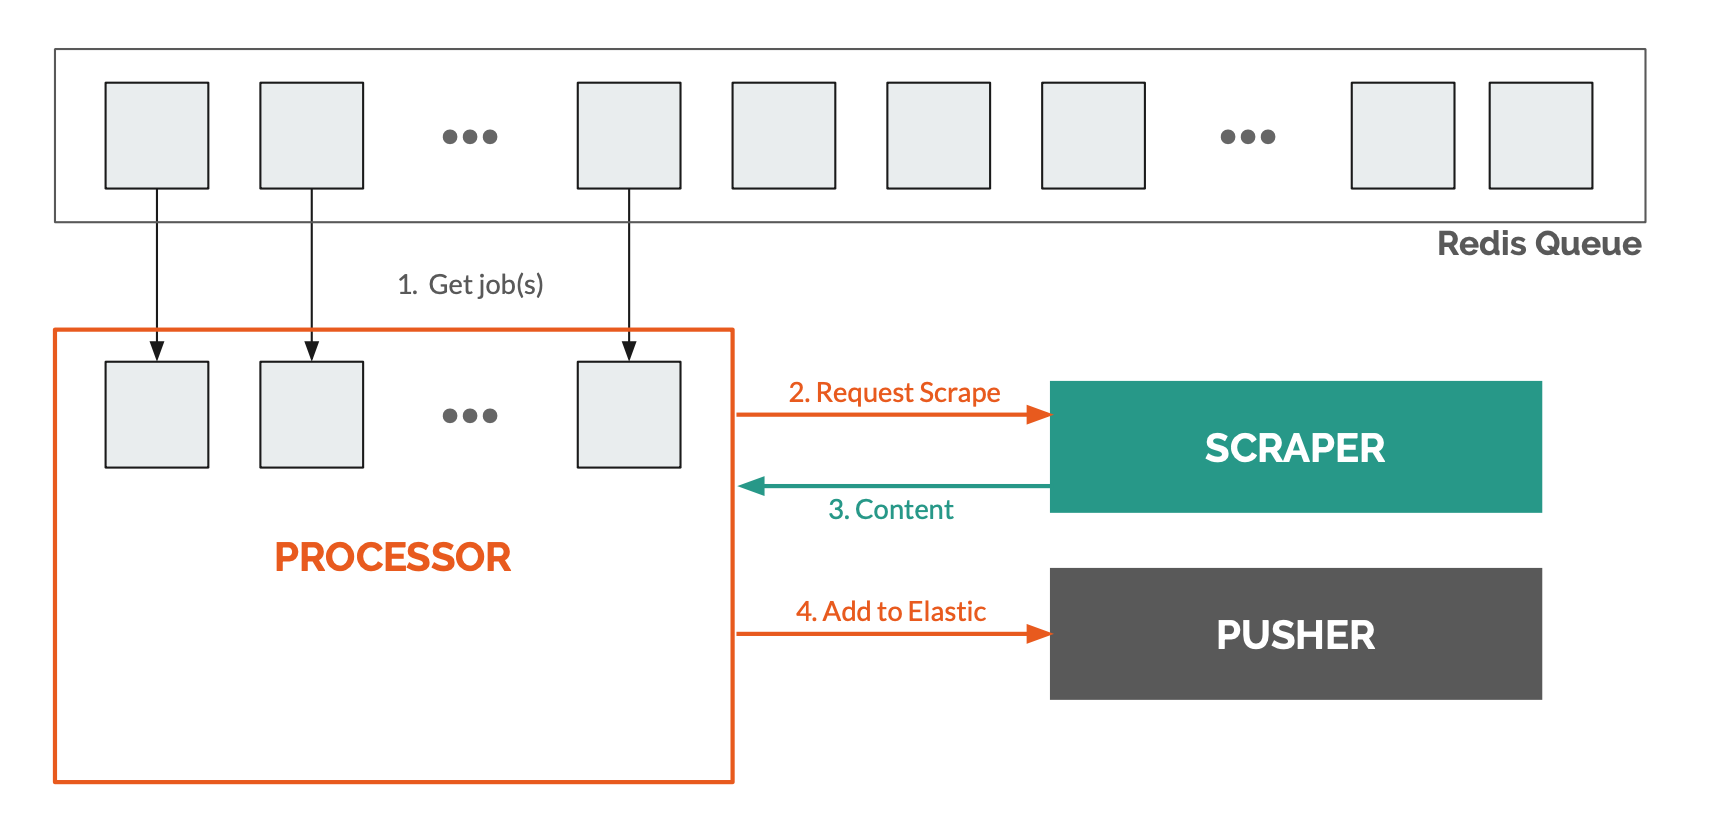
\includegraphics[width=\linewidth]{images/processor.png}
  \caption{Abarbeiten von Scrap-Jobs}
  \label{processor:image:processor}
\end{figure}


\subsection{Abfragen von RSS Feeds}
Die RSS Feeds werden zentral in der Datenbank des Collectors gespeichert und sind über eine REST-API verfügbar.
Um nicht bei jeder Aktualisierung der RSS-Feeds alle sich im Feed befindenden Dokumente zu indizieren, wird in Redis als Schlüssen-Wert-Paar die URL des RSS Feed und der Zeitpunkt an dem er zuletzt abgefragt wurde gespeichert.
Der Zeitpunkt des letzten Abfragens wird an die RSS Komponente von Elastifeed weiter gegeben, sodass nur neue Einträge zurückgeliefert werden.
Anschließend werden die Elemente am Ende der Warteschlange hinzugefügt.
Der Processor koordiniert diesen Prozess in einem konfigurierbaren Zeitabstand.

\begin{minted}[breaklines]{python}
for feed in parsed:
    # Get last parsed timestamp out of redis or assume it was scraped on 10.05.2019
    last_time_raw = await redis.execute("get", f"feed:{feed['link']}") or b"2019-05-10T00:00:00.000000+00:00"
    last_time = datetime.fromisoformat(last_time_raw.decode("UTF-8"))
    for job in await rss.get(feed["link"], last_time):

        # Add to queue
        await redis.execute("RPUSH", "queue:items", dumps(QueueElement(
            url=job.url,
            title=job.title,
            feed_url=feed["link"],
            categories=[],
            indexes=[f"user-{u['id']}" for u in feed["users"]]
        )))

    # Update timestamp
    await redis.execute("set", f"feed:{feed['link']}", datetime.now(timezone.utc).astimezone().isoformat())
\end{minted}
